\chapter{TensorFlow}
\label{cha:TensorFlow}

TensorFlow repräsentiert eine Bibliothek für Machine Intelligence. 
Historisch gesehen entstand TensorFlow in der Google Brain Abteilung.
Das Projekt wird als Open Source Projekt weiterentwickelt, wobei das Projekt von Google weiterhin gepflegt wird. 
Das Offenlegen des Projekts führt dazu, dass auch Personen außerhalb von Google die Möglichkeit bekommen, die Bibliothek zu verwenden sowie dazu etwas beitragen zu können. \newline

\noindent
Das Hauptkonzept in TensorFlow sind sogenannte Tensoren, welche einen Graphen durchlaufen. 
%Diese Tensoren werden während ihrem durch lauf verändert und wieder neu zusammengesetzt. 
Der Graphen selbst stellt damit einen Datenflussgraphen dar, welcher Knoten beinhaltet. 
Diese Knoten bilden numerische Operationen ab.
Der Informationsaustausch zwischen den Knoten geschieht mit multidimensionalen Arrays, den so genannten Tensoren.
TensorFlow bietet wie andere Bibliotheken die Möglichkeit die Berechnungen auf eine Grafikkarte auszulagern.
Zusätzlich sind weite Routinen eingebaut, damit das Trainieren über mehrere Grafikkarten verteilt werden kann sowie auf weitere Computer. \newline

\noindent
TensorFlow steht für mehrere Programmiersprachen zur Verfügung, welche offiziell unterstützt werden, wobei es noch mehr durch die Open Source Gemeinschaft unterstützte Sprachen gibt.
Den Hauptbereich stellt die Python API dar, welche auch die vollständigste Implementierung darstellt. 
Der Kern von TensorFlow ist mit C++ und Python implementiert und wurde sehr stark optimiert, um eine sehr gute Performanz zu erzielen.
Die Python API wird im Umfeld von TensorFlow dazu verwendet, um einen Graphen zu erstellen, zu trainieren und zu testen. 
Durch die Verwendung von Python besteht die Möglichkeit sehr schnell Änderungen am Graphen durchzuführen und nicht erst ganze Applikationsstrukturen zu übersetzten, damit ein Ergebnis der Änderung ersichtlich wird. 
Dieser Graphen wird nach seiner Trainingsphase exportiert und beinhaltet alle Knoten sowie die dazugehörigen Gewichtungen. 
Die C++ API sowie die Java API und GO API zielen auf eine sehr effiziente Ausführung ab.
Durch die Verwendung des trainierten Graphen kann dieser auch auf mobilen Plattformen eingesetzt werden.

\subsection{Graphs/Dataflowgraph}

\begin{figure}

\lstset{language=Python}
\begin{lstlisting}
import tensorflow as tf

b = tf.Variable(tf.zeros([100])) 
	# 100-d Vektor, initialisiert mit 0
W = tf.Variable(tf.random_uniform([784,100],-1,1)) 
	# 784x100 Matrix w/rnd vals
x = tf.placeholder(name="x") 
	# Platzhalter für Eingangsdaten
relu = tf.nn.relu(tf.matmul(W, x) + b) 
	# Relu(Wx+b) Aktivierungsfunktion mit impliziter Addition
C = [...] 
	# Kostenfunktion und noch weitere Knoten
s = tf.Session()
for step in xrange(0, 10):
	input = ...construct 100-D input array ... 
		# Erstellen eines 100-d Vektor mit den Eingangsdaten
	result = s.run(C, feed_dict={x: input}) 
		# Graphen mit den Eingangsdaten ausführen
	print step, result 
		# Ausgabe des Berechneten Resultats
\end{lstlisting}

	\caption{TensorFlow Codefragment zur Definition eines Teils des Graphen}
	\label{fig:SimpleFragmentGraphDefinition}
\end{figure}

\begin{figure}

	\centering

\begin{tikzpicture}

	\node[neuron] (x) {x};
	\node[neuron,below=of x] (w) {W};
	
	\node[group,fit={(x) (w)}] (gr1) {};
	
	\node[neuron,right=of x] (MatMul) {MatMul};
	\node[io,below=of MatMul] (b) {b};
	
	\node[group,fit={(x) (MatMul)},right=of x] (gr2) {};
	
	\node[neuron,right=of MatMul] (Add) {Add};
	
	\node[neuron,right=of Add] (ReLU) {ReLU};
	
	\node[neuron,right=of ReLU] (more) {...};
	
	\node[neuron,right=of more] (C) {C};
	
	\draw[conn] (x) -- (MatMul);
	\draw[conn] (w) -- (MatMul);

	\draw[conn] (MatMul) -- (Add);
	\draw[conn] (b) -- (Add);
	
	\draw[conn] (Add) -- (ReLU);
	\draw[conn] (ReLU) -- (more);

	\draw[conn] (more) -- (C);

\end{tikzpicture}

	\caption{Der resultierenden Teilgraph aus dem Codefragment aus Abbildung \ref{fig:SimpleFragmentGraphDefinition} nach dem Beispiel in \cite{wp2015tensorflow}}
	\label{fig:SimpleFragmentGraphPic}
\end{figure}

Ein TensorFlow Graph kann wie in Abbildung \ref{fig:SimpleFragmentGraphDefinition} beschrieben werden.
Dieser wurde zum Beispiel mit der Python API erstellt.
Im Gesamten mit den Knoten und den Verbindungen ergibt sich ein Datenfluss, diese beinhaltet alle erforderlichen Komponenten auch für das per sistieren und aktualisieren der Daten.
Dies sind Erweiterungen für den Hauptgraphen und beinhalten auch Logik für Schleifenverwaltungen.
Ein Knoten in einem Graphen besitzt $0$ bis $n$ Ein und Ausgänge und besitzt eine Kernfunktion. 
Zu den Datenhauptfluss mit den Tensoren gibt es zusätzlich spezielle Verbindungen, welche "control dependencies" genannt werden. 
Anhand dieser Verbindungen werden keine Daten im Sinne der Tensoren übertragen, sondern werden benützt um Abhängigkeiten zu definieren, um zum Beispiel eine Ausführung in einem anderen Knoten vor einem anderen zu definieren.
So muss der Quellknoten mit der Ausführung abgeschlossen haben bevor der darauf wartende mit der Ausführung beginnt. \cite{wp2015tensorflow}

\subsection{Operation}

Die Operation stellt in jedem Knoten den Kern dar, wie zum Beispiel eine Matrix Multiplikation oder eine Addition.
In TensorFlow selbst gibt es einen Unterschied zwischen Operation und Kernel.
Operationen besitzen Attribute, welche spätestens zum Zeitpunkt der Grapherstellung bekannt sein müssen. 
Ein solches Attribut wäre zum Beispiel, \textit{um eine Operation Polymorph für Datentypen zu ermöglichen}. 
Der Kernel selbst ist die Implementierung der Operation selbst. 
Dieser kann auf verschiedenen Geräten ausgeführt werden wie CPU oder GPU.
Die Operationen und die dazugehörigen Kernel werden über einen Registrierungsmechanismus zur Verfügung gestellt. 
Diese Sammlung an Operationen kann auch Erweitert werden. \cite{wp2015tensorflow} 

\subsection{Sessions}

Die Session repräsentiert die Laufzeit für einen Graphen. 
Dieser Session wird ein Graphen übergeben, welcher erst initialisiert werden muss. 
Ohne die Initialisierung ist der Knoten und Verbindungen würde die weitere Ausführung mit diesem nichts produzieren, da alle Werte $0$ sind. 
Diese stellt eine weitere Funktion zur Verfügung \textit{Run}. 
Der Run-Funktion wird eine Liste Endknoten übergeben welche berechnet werden sollen und die zu dem initialisierten Graphen gehören. 
Die Platzhalter Tensoren werden mit Daten verknüpft und so in den Graphen gereicht. 
In den Meisten fällen wird ein Graphen einmal erstellt und mehrfach ausgeführt. \cite{wp2015tensorflow} 

\subsection{Tensor}

In TensorFlow ist ein Tensor ein typisiertes multidimensionales Array. 
Die verwendbaren Typen reichen von Datentypen mit Vorzeichen und ohne sowie bis hin zu Doubles und Zeichenketten. \cite{wp2015tensorflow} 

\section{Bibliotheksinhalt}

\subsection{Datentypen}

TensorFlow besitzt eine große Anzahl an Datentypen die verwendet werden können. 
Dies reicht von Grunddatentypen wie 'Boolean' und 'String' bis hinzu verschiedene Integer Datentypen. 
Diese stehen in verschiedene Wertebereichen zur Verfügung. 
So gibt es Gleitkommazahlen mit unterschiedlicher Genauigkeit, wie 16-bit was für halbe Genauigkeit steht aber auch bis zu 64-bit Genauigkeit reicht, was einer doppelten Genauigkeit entspricht. 
Der Grund für diese verschiedenen Anzahlen an Datentypen ist, dass diese zur Optimierung verwendet werden können. 
Ein trainiertes Netzwerk welches nie in den Wertebereich von 64-bit signierte Integers gekommen ist, wird diese möglicherweise nie benötigen. 
In diesem Fall können die Wertebereiche reduziert werden, auf zum Beispiel 32-bit signierte Integer und somit die Berechnungen hochperformanter ausgeführt werden. \cite{TensorFlow}

\subsection{Operationen}

\subsubsection{Konstanten und Zufallswerte}

\paragraph{Konstanten} stehen in TensorFlow vordefiniert zur Verwendung.
Diese stellen initialisierte Tensoren für den ersten Trainingsdurchlauf zur Verfügung.

\begin{itemize}
	\item \textit{tf.zeros} erstellt einen Tensor mit angegebenen Dimension bestehend aus $0$ und von einem Datentypen. 
	\item \textit{tf.zeros\_like} gibt einen Tensor zurück, welcher die selbe Dimensionen wie der gegeben besitzt.
	Alle Werte in diesem Tensor sind aber auf $0$ gesetzt.
	In diesem Zuge kann der Datentyp mit angepasst werden, wenn nur die Dimensionen übernommen wenden sollen.
	\item \textit{tf.ones} agiert genau wie der Tensor \textit{tf.zeros} mit dem unterschied dass alles mit $1$ gefüllt ist.
	\item \textit{tf.ones\_like} repräsentiert das selbe wie \textit{tf.zeros\_like} nur mit $1$.
	\item \textit{tf.fill} wird zu der Dimension noch ein Skalar mit gegeben, für die Werte die ausgefüllt werden sollen.
	\item \textit{tf.constant} liefert einen Tensor mit selbst definierbaren Werten. 
	Diese Werte können eine Liste sein sowohl als auch eine einzelner Wert welcher überall eingefügt werden soll. 
\end{itemize}

\paragraph{Sequenzen} können verwendet werden um einen Wertebereich in eine bestimmte Anzahl an Werte zu zerteilen und diese als Tensor in das System einfließen zu lassen.

\begin{itemize}
	\item \textit{tf.lin\_space} generiert einen eindimensionalen Tensor vom Datentypen $32$ oder $64$-bit Gleitkommazahlen, mit einer bestimmten Folge.
	Diese beginnt mit dem Startwert und endet mit dem Endwert. 
	Die Werte dazwischen werden gleichmäßig verteilt erstellt. 
	\item \textit{tf.range} erstellt wie \textit{tf.lin\_space} einen eindimensionalen Tensor mit Skalarwerten. 
	Die Folge beginnt mit einem Startwert und erweitert sich um ein Delta bis zum Endwert, welcher nicht Teil der Folge ist. 
\end{itemize}

\paragraph{Zufallswerte} werden im Bereich von maschinellen Lernens sehr häufig benötigt. 
So werden meist der Startzustand mithilfe von Zufallszahlen hergestellt. 

\begin{itemize}
	\item \textit{tf.random\_normal} liefert einen Tensor mit Zufallswerten anhand einer Normalverteilung (Gaussian). 
	Die Dimension des Ergebnistensors muss spezifiziert werden, der Meridian, Standardabweichung sowie der resultierende Datentyp können angegeben werden. 
	\item \textit{tf.truncated\_normal} verhält sich gleich zu \textit{tf.random\_normal} mit dem unterschied, dass Werte die größer sind als $2$-mal die Standardabweichung, ignoriert werden und ein neuer Wert ausgewählt wird.
	\item \textit{tf.random\_uniform} generiert einen Tensor in welchem Werte gleich Wahrscheinlich vorkommen.
	Die Werte werden aus dem spezifizierten Wertebereich genommen, wobei diese exklusive der oberen Grenze ist, wie zum Beispiel '$[0, 1)$'.
	\item \textit{tf.random\_shuffle} erstellt selber keine neuen Werte sondern, mischt einen Tensor anhand seiner ersten Dimension durch. 
	\item \textit{tf.random\_crop} liefert einen zufälligen Teil eines Tensors mit der selben Anzahl an Dimensionen und aber mit der spezifizierten Größe.
\end{itemize} \phantom \newline

\noindent
Einige dieser Funktionen benötigen sogenannte Seed-Werte, welche den Startwert der Zufallszahlen zerstreuen sollen sowie die Folge selbst. 
Im Falle von TensorFlow beruht dies auf zwei Werten, einer wird für den Graphen spezifiziert, der zweite wird für die Operation selbst spezifiziert. 
Der Wert für den Graphen kann mit \textit{tf.set\_random\_seed} gesetzt werden. 
Für weiter Informationen steht die online Dokumentation zur Verfügung. \footnote{Online Dokumentation: Constants, Sequences, and Random Values  \url{https://www.tensorflow.org/api_guides/python/constant_op}}

\subsubsection{Variables}

Variablen geben bei jedem Durchlauf einen Tensor ab.
Dieser Wert ändert sich nicht, außer ihm wird eine neuer Wert zugewiesen. 

\subsubsection{Transformationen}

\paragraph{Casting} bietet die Möglichkeit wie in anderen Programmiersprachen Typen zu konvertieren. 
Diese Operation muss in den Graphen eingepflegt werden, da keine impliziten Konvertierungen durchgeführt werden. 
Es kann jeder Tensor konvertiert werden, sowie eine Zeichenfolge in eine Zahl. 
Bei diesem Vorgang kann ein Fehler entstehen, welcher in \textit{TypeError} resultiert.

\paragraph{Shapes und Shaping} liefert die Gestalt eines Tensors, bietet aber auch die Möglichkeit diese zu ändern. 
\begin{itemize}
	\item \textit{tf.shape} liefert eine genaue Aufschlüsselung des Tensors mit der Dimension und der Tiefe.
	\item \textit{tf.size} repräsentiert die Anzahl an Elementen in einem Tensor. 
	Diese Anzahl ergibst sich aus den konkreten Werten.
	\item \textit{tf.rank} verhält sich ähnlich zu \textit{tf.size} mit dem unterschied, dass die Anzahl der Felder Vertiefung gezählt wird.
	\item \textit{reshape} wird verwendet um Tensoren in eine neue Struktur zu bringen. 
	Dabei kann für das einebnen der Dimensionen eine Kurzschreibweise verwendet werden mit $-1$ als Zielausführung der Gestalt.
	\item \textit{tf.squeeze} entfernt ganze Dimensionen aus dem gegebenen Tensor. 
	Ohne Achsen Angabe werden alle Dimensionen mit der Größe $1$ entfernt oder es werden die spezifizierten Dimensionen herausgenommen.
	\item \textit{tf.expand\_dims} gliedert wider um Dimensionen in einen Tensor ein. 
	Im Standard an der Indexstelle $0$, außer es wurde spezifiziert.
\end{itemize}

\paragraph{Slicing und Joining} wie in diversen Programmiersprachen unterstützt auch TensorFlow das Teilen und Zusammenfügen von Daten und aber hier im Speziellen mit Tensoren. 
Diese Operationen reichen von einfachen Slicing Operationen über Transponieren bis hin zu dem Verketten von Tensoren, dabei kann definiert werde Anhand welcher Achse der Dimensionen die Operation ausgeführt werden soll.

%\paragraph{Fake quantization} => zu viel
\phantom \newline

\noindent
Weiter Informationen befinden sich in der online Dokumentation. \footnote{Online Dokumentation: Tensor Transformations \url{https://www.tensorflow.org/api_guides/python/array_ops}}

\subsubsection{Mathematik} 

\paragraph{Arithmetische Operationen} stellen die mathematischen Grundoperationen dar. 
Diese können teilweise in Kurzschreibweisen verwendet werden, wie zum Beispiel die Addition. 
Diese kann entweder als explizite Operation \textit{tf.add(x, y)} verwendet werden aber auch Implizit bei der Addition $+$ von einem Tensor mit einem Bias-Tensor.

\paragraph{Basis Funktionen} ergänzen die arithmetischen Operationen um Standardfunktionen. 
Zu diesen Funktionen zählen die Berechnung der Absolutwerten in einem Tensor sowie eine Exponentialfunktion. 

\paragraph{Matrizen Funktionen} werden am häufigsten benötigt, da Tensoren im Grunde Matrizen sind und somit diese geändert werden können. 
\begin{itemize}
	\item \textit{tf.matmul} führt eine Matrizenmultiplikation aus. 
	Diese Operation findest meist in voll Vernetzten Neuronen Verwendung, wenn der übergebene Tensor mit der Gewichtung multipliziert wird. 
	\item \textit{tf.eye} erzeugt eine Identitätsmatrix, in welcher alle Werte an der Diagonale $1$ sind und alle anderen $0$. 
\end{itemize}

Zu diesen Funktionen existieren noch weitere die zur Lösung von Gleichungen verwendet werden können. 
Diese Gleichungen müssen in Matrizenschreibweise im Tensor abgebildet sein. 

\paragraph{Komplexe Zahlen} können verwendet werden und Operationen mit ihnen in de Graphen eingepflegt werden. 

\paragraph{Reduzierungsoperationen} kommen meist dann zum Einsatz, wenn der Unterschied zwischen dem Ergebnis und dem erwarteten Ergebnis festgestellt werden soll. 
\begin{itemize}
	\item \textit{tf.reduce\_sum} berechnet die Summe aller Werte in einem Tensor.
	\item \textit{tf.reduce\_mean} berechnet die Summe aller Werte an der Diagonale eines Tensors. 
	\item \textit{tf.reduce\_max} reduziert einen Tensor auf die maximal Werte in der letzten Dimension und reduziert dabei den Rang um eins.
\end{itemize}

\noindent
Zu diesen gibt es noch weiter, welche in diversen Fällen benötigt werden wenn zum Beispiel Wahrheitswerten reduziert werden sollen. \newline

\noindent
Die Anzahl an mathematischen Funktionen ist um einiges sehr viel Größer als die hier erwähnten. 
Diese hier repräsentieren lediglich die meist verwendeten Operationen. 
Für weiter Informationen steht die online Dokumentation zur Verfügung. \footnote{Online Dokumentation: Math \url{https://www.tensorflow.org/api_guides/python/math_ops}}

\subsubsection{Flusskontrolle}

\paragraph{Flusskontrolle} sind Operationen die den Ablauf in dem Graphen beeinflussen. 
Dies können Bedingungen sein, wie im Sinne von \textit{if (Bedingung){...} else {}} aber auch \textit{switch (Term) { case '0': ...; break;}} Bedingungen sein. 
In beiden Fällen müssen die Auszuführenden Verzweigungen als Funktionen vorliegen. 
Zusätzlich gibt es noch eine \textit{While} und eine \textit{For} Schleife. 
Zu beachten ist, dass diese Operationen und weiter den Fluss durch den Graphen stark beeinträchtigen können.

\paragraph{Logik Operatoren} können verwenden werden um Vergleiche zwischen Tensoren durchzuführen. 
Diese werden aber als Logik Operationen ausgeführt und liefern immer Wahrheitswerte, wie eine Logische Und-Verknüpfung auf Binärebene.

\paragraph{Vergleichsoperatoren} neben den Logischen Operatoren stehen weitere Vergleichsoperatoren zur Verfügung. 
Hierzu zählen \textit{tf.equal} sowie die verneinte Variante, \textit{tf.less} und \textit{tf.greater} mit jeweils einer gleich Version. 
Diese Operatoren geben wiederum einen Tensor mit Wahrheitswert aus.

\paragraph{Debugging Operationen} ermöglichen es in den Graphen Kontrollstrukturen einzubauen, welchen auf diverse Bedingungen reagieren.
So kann Überprüft werden ob ein Tensor Werte mit undefinierten Zustand beinhaltet. 
Die Funktion \textit{tf.Print} ermöglicht es Tensoren auszugeben wenn diese Funktion im Graphen evaluiert wird. 
Aktuell sind die Möglichkeiten eine Graphen zu debuggen relative eingeschränkt, da der Graphen ist grundsätzlich einsehbar aber schwer zu verstehen in seiner rohen Darstellung.
\footnote{Online Dokumentation: Control Flow \url{https://www.tensorflow.org/api_guides/python/control_flow_ops}}

\subsubsection{Images}

\paragraph{Encodieren und Decodieren} von Bilddateien wird TensorFlow direkt unterstützt.
Dabei können Bildern von den Datentypen Gif, Jpeg und PNG gelesen werden, sowie das erstellen von Bildern in diese Datentypen, ausgenommen Gif. 
In allen Fällen wird das Bild als Zeichenkette mit Pfad angegeben. 

\paragraph{Größenänderung} von Bilder sind erforderlich, da Bilder die eingelesen werde zu große sind und somit in die Struktur des Graphen nicht eingelesen werden können. 
Für die Größenänderung stehen mehrere Implementierungen zur Verfügung mit unterschiedlichen Algorithmen und vorgehen im Hintergrund.

\paragraph{Beschneiden} wird dann benötigt wenn aus einem Bild ein Teil herausgenommen werden soll. 
Zum herausnehmen stehen wiederum mehrere Operationen zur Verfügung, welche mit umschließende Boxen arbeiten oder wie viel Prozent von der Mitte des Bildes aus genommen werden soll.

\paragraph{Flippen, Rotieren und Transponieren} ermöglicht es Bilder zu Verändern, so dass es für einen Menschen mehr oder weniger immer noch die selbe Bedeutung hat aber nicht mehr für einen Computer. 
Für diesen stellt ein Rotiertes oder Gespiegeltes Bild ein neues Bild dar. 
Diese Technik wird beim Trainieren von Bilderkennungen eingesetzt um zum Beispiel aus geringen Datenmengen die zum Trainieren verfügbar sind, mehrere zu generieren.
\phantom \newline

\noindent
Zusätzlich gibt es noch die Möglichkeit die Farbkanäle des Bildes zu ändern sowie das Bild nachzujustieren. 
\footnote{Online Dokumentation: Images \url{https://www.tensorflow.org/api_guides/python/image}}

\subsubsection{Input und Readers}

\paragraph{Platzhalter} werden benötigt um einen Graphen zu erstellen. 
Ohne Platzhalter wäre es nicht möglich Daten in den Graphen zu bekommen. 
Diese müssen zur Ausführungszeit durch richtige Daten ersetzt werden, was mit Hilfe von einem Schlüssen-Wert-Paars erfolgt. 

\paragraph{Readers} ermöglichen direkt aus dem Dateisystem Daten zu laden. 
Dabei stehen spezifizierte Reader zur Verfügung welche die direkt Tensoren ausliefern sowie Zeile für Zeile  oder ganze Dateiinhalte liefern. 

\paragraph{Konvertierungsoperationen} ermöglichen es Dateien die mit TensorFlow Readers gelesen wurden weiter zu verarbeiten, so kann eine CSV Datei decodiert verwendet werden.
\phantom \newline

\noindent
Des Weiteren sind Protokoll Buffer sowie Queues implementiert die zum Vorverarbeiten von Daten sind.
\footnote{Online Dokumentation: Input und Readers \url{https://www.tensorflow.org/api_guides/python/io_ops}}

\subsubsection{Neuronale Netzwerke}

Neuronale Netzwerke sind eine Spezialisierung des Gebietes des maschinellen Lernens. 
So bietet TensorFlow eine breite Unterstützung beziehungsweise eine große Implementierungsvielfalt für diesen Typ an. 

\paragraph{Aktivierungsfunktion} repräsentieren den Ausgang eines Neurons dar, dabei existieren aus der Vergangenheit heraus einige Ansätze für diesen Bereich eines Neuronalen Netzwerkes. 
\begin{itemize}
	\item \textit{tf.sigmoid} ist eine der bekanntesten und ältesten diesen Typs.
	Diese Funktion hat im Punkt $0$ einen Aktivierungswert von $0.5$ und besitzt zwei Beschränkungen. 
	Im negativen Zahlenbereich auf der X-Achse wird die Funktion mit $0$ der Grenzwert definiert und im positiven Zahlenbereich auf der X-Achse wird diese mit dem Grenzwert von maximal $1$ definiert. 
	Ein negativer Wert führt somit zu einem geringen Aktivierungswert, welcher sich im Negativen an $0$ annähert sowie im Positiven an $1$.
	Im Diagramm \ref{fig:Sigmoide Aktivierungsfunktion} befindet sich dies Funktion mit ihren Grenzwerten. 
\begin{figure}
	\centering
	\resizebox {\linewidth} {5cm} {
	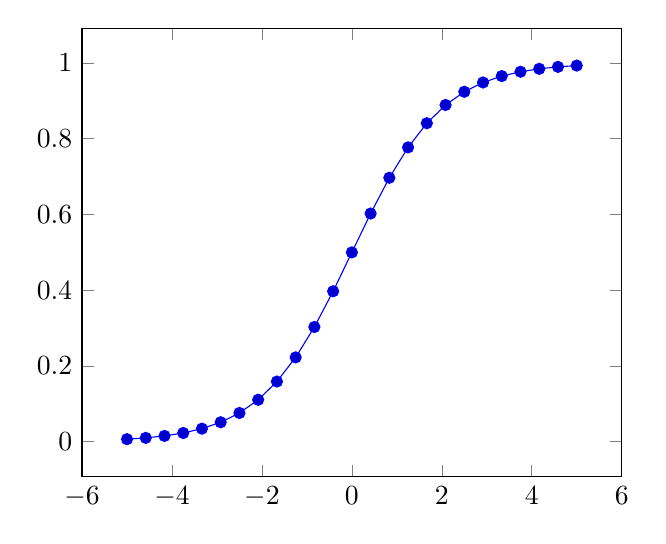
\begin{tikzpicture}
	\begin{axis}

		\addplot expression { 1/(1+exp(-x) };

	\end{axis}
	\end{tikzpicture}
	}
	\caption{Sigmoide Aktivierungsfunktion}
	\label{fig:Sigmoide Aktivierungsfunktion}
\end{figure}

	\item \textit{tf.relu} ersetzt mittlerweile immer mehr die Sigmoide Version. 
	Ein Grund dafür ist, dass die Berechnung mit Sigmoidefunktionen Ressourcen intensive ist. 
	Die rektifiziert lineare Funktion ist sehr viel einfacher, denn Werte unter $0$ werden als $0$ weiter gegeben und Werte darüber linear. 
	Somit resultiert ein Eingangswert von $-0.1$ in einer $0$ und ein Wert von $0.5$ in $0.5$.
	Wie im Diagramm \ref{fig:rektifiziert lineare Aktivierungsfunktion} ersichtlich ist, führt dies bei einem negativen Wert dazu, dass eine Multiplikation mit der Gewichtung in der nächsten Ebene ebenfalls in einer $0$ sich repräsentiert und somit in der Addition ignoriert wird.
\begin{figure}
	\centering
	\resizebox {\linewidth} {5cm} {
	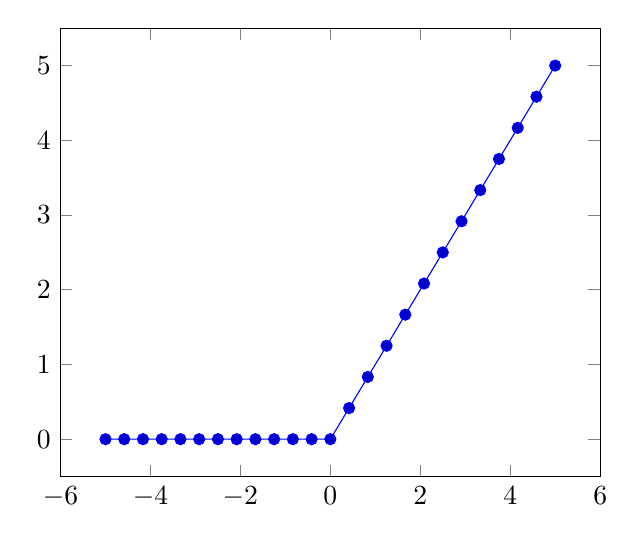
\begin{tikzpicture}
	\begin{axis}

		\addplot expression { max(0, x)};

	\end{axis}
	\end{tikzpicture}
	}
	\caption{rektifiziert lineare Aktivierungsfunktion}
	\label{fig:rektifiziert lineare Aktivierungsfunktion}
\end{figure}

	\item \textit{tf.tanh} genannt als Hyperbolic Tangent gehört ebenfalls zu den grundlegenden Aktivierungsfunktionen. 
	Der Unterschied zwischen dieser Funktion und der Sigmoiden Aktivierungsfunktion ist, dass der untere Grenzwert nicht bei $0$ liegt sondern bei $-1$. 
	Im Diagramm \ref{fig:Hyperbolic Tangents Aktivierungsfunktion} ist zu sehen, wo sich der Wendepunkt befindet, was im Falle des Hyperbolic Tangent in der Koordinate $x = 0, y = 0$ ist. 
\begin{figure}
	\centering
	\resizebox {\linewidth} {5cm} {
	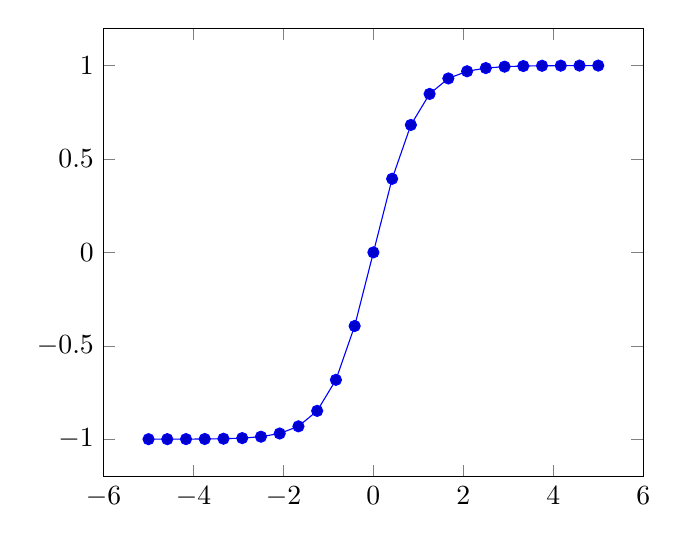
\begin{tikzpicture}
	\begin{axis}

		\addplot expression { tanh(x)};

	\end{axis}
	\end{tikzpicture}
	}
	\caption{Hyperbolic Tangents Aktivierungsfunktion}
	\label{fig:Hyperbolic Tangents Aktivierungsfunktion}
\end{figure}
\end{itemize}
\phantom \newline

\noindent
Zu diesen Aktivierungsfunktion stehen noch einige weiter zur Verfügung, die ausführlich getestet gehören. 
Im Grunde könnte jede Funktion verwendet werden, doch jede besitzt eine Eigenheit und beeinflusst so den gesamten Graphen. 

\paragraph{Faltung Operationen} werden bei Bilderkennungen unter anderem deshalb verwendet, da sie eine Operation auf einen Stapel an Daten gleichzeitig anwenden. 
So wird wird ein Fenster über ein Bild geschoben und auf jedes Bild wird in dem selben Fenster die Operation durchgeführt. 
Diese Operation generalisiert die darunterliegenden Daten, so als ob sie auf Etwas reagiert hätten. 
Dies entspricht dem als ob ein Auge auf etwas reagiert hätte. 
\textbf{TODO: Diagramm}
\begin{itemize}
	\item \textit{tf.nn.conv2d} steht für zweidimensionale Bilder zur Verfügung. 
	\item \textit{tf.nn.conv3d} ermöglicht es mit dreidimensionale Objekte zu arbeiten.
\end{itemize}

Des Weiteren stehen noch weitere spezialisierte Versionen implementiert zur Verfügung.

\paragraph{Bündelung} wird verwendet um Daten zu vereinfachen. 
Eine Faltungsoperation führt dazu, dass aus einem Bild viel erzeugt werden mit unterschiedlichen Filtern. 
Eine Bündelung ermöglicht einen Vereinfachung der Bilder, sodass sie vereinfacht werden und dabei die Schlüsselinformationen aber dennoch erhalten bleiben. 
Diese Technik wurde zu früheren Zeiten eingesetzt, um Computerressourcen zu sparen, da diese nicht so leistungsfähig waren wie sie aktuell sind. 
TensorFlow bietet mehrere Umsetzungen, so kann der Maximalwert aus der Filtermatrix übernommen werden wie aber auch der Mittelwert. 

\paragraph{Verluste} beschreiben wie sehr ein Ergebnis von dem erwarten Ergebnis entfernt ist. 
Diese Art der Verlust Feststellung wird bei Regression Probleme benötigt aber auch regulieren im generellen.
\begin{itemize}
	\item \textit{tf.nn.l2\_loss} berechnet einen Wert, welcher den Inhalt des Tensors repräsentiert. 
	Im Falle dieser Implementierung wird keine Wurzel des Quadrats berechnet, sondern es werden die Werte nur addiert und durch $2$ dividiert.
	\item \textit{tf.nn.log\_poisson\_loss} berechnet den Logarithmischen-Wahrscheinlichkeitsverlust zwischen einem Ergebnis und einem erwarteten Ergebnis. 
	Diese Methode liefert im Normalfall nicht den exakten Verlust, was für Optimierungen nicht das Problem ist. 
	Sollte trotzdem ein genaueren Wert berechnet werden zum Vergleichen von Verlusten, muss die aufwändige Stirling Approximation aktiviert werden. 
\end{itemize}

\paragraph{Klassifizierungen} repräsentieren eine großen Bereich des maschinellen Lernens. 
TensorFlow besitzt deshalb mehrere Hilfsfunktionen, welche das arbeiten mit Klassifizierungen erleichtert. 
\begin{itemize}
	\item \textit{tf.nn.softmax} bildet alle Ergebnisse auf einen prozentualen Bereich ab. 
	So ergeben alle möglichen Ausgänge in Summe 100\%, was soviel bedeutet das ein Ergebnis eine gewisse Wahrscheinlichkeit besitzt. 
	\item \textit{tf.nn.softmax\_cross\_entropy\_with\_logits} bietet einem die Möglichkeit auf nicht skalierte Daten ein Ergebnis zu Berechnen, welches eine \textit{tf.nn.softmax} Berechnung liefern würde. 
	Zusätzlich wird eine weitere so genannte 'cross entropy' Operation ausgeführt, wo das Ergebnis für Optimierungen benötigt wird. 
	Die gesamte Methode berücksichtigt Spezialfälle im gesamten Prozess, welche schwer manuell ab zu berücksichtigen sind. 
\end{itemize}

\noindent
Zu diesen existieren noch weitere Implementierungen mit weiteren Eigenheiten, welche in diversen Situation möglicherweise einen Vorteil bieten. 

%\paragraph{Wiederkehrend Neuronale Netzwerke} 

\noindent
Des Weiteren gibt es Implementierungen für Wiederkehrende Neuronale Netzwere und weiter Dinge in diesem Themengebiet. 
\footnote{Online Dokumentation: Neural Network \url{https://www.tensorflow.org/api_guides/python/nn}}

\subsubsection{Running Graphs}

\paragraph{Session}

\subsubsection{Training}

\paragraph{Optimizers}

\paragraph{Gradient Computation}

%\subsection{Probleme}

%\subsubsection{NaN Problem}

\subsection{TensorBoard}

\paragraph{Graph}
\paragraph{Event}
\paragraph{Histogram} https://duckduckgo.com/?q=tensorboard+histogram&ia=qa